\chapter{Results and Analysis} \label{ch:results-analysis}

We demonstrate the output of the Frangi filter on our samples after running a multiscale technique with $N=20$ scales with a stricter anisotropy $\beta = .35$ and $\gamma=0.5$,
with scales spaced logarithmcally from $\sigma_1 = 2^{-1}$ to $\sigma_N = 2^{3.5}$, performing glare and cut removal in preprocessing, and using a discrete gaussian kernel and dilation border of 20.

\section{Sample visual output}
In \cref{fig:output-montage-example1} and \cref{fig:output-montage-example2} we take a partial look at the Frangi output for two particularly well-behaved samples. In the top-left, the preprocessed placenta is shown. In the top-right, the maximum of the Frangi output over $N$ scales. The bottom left and right images are simple segmentation strategies of merging the result.

\begin{figure} \centering
  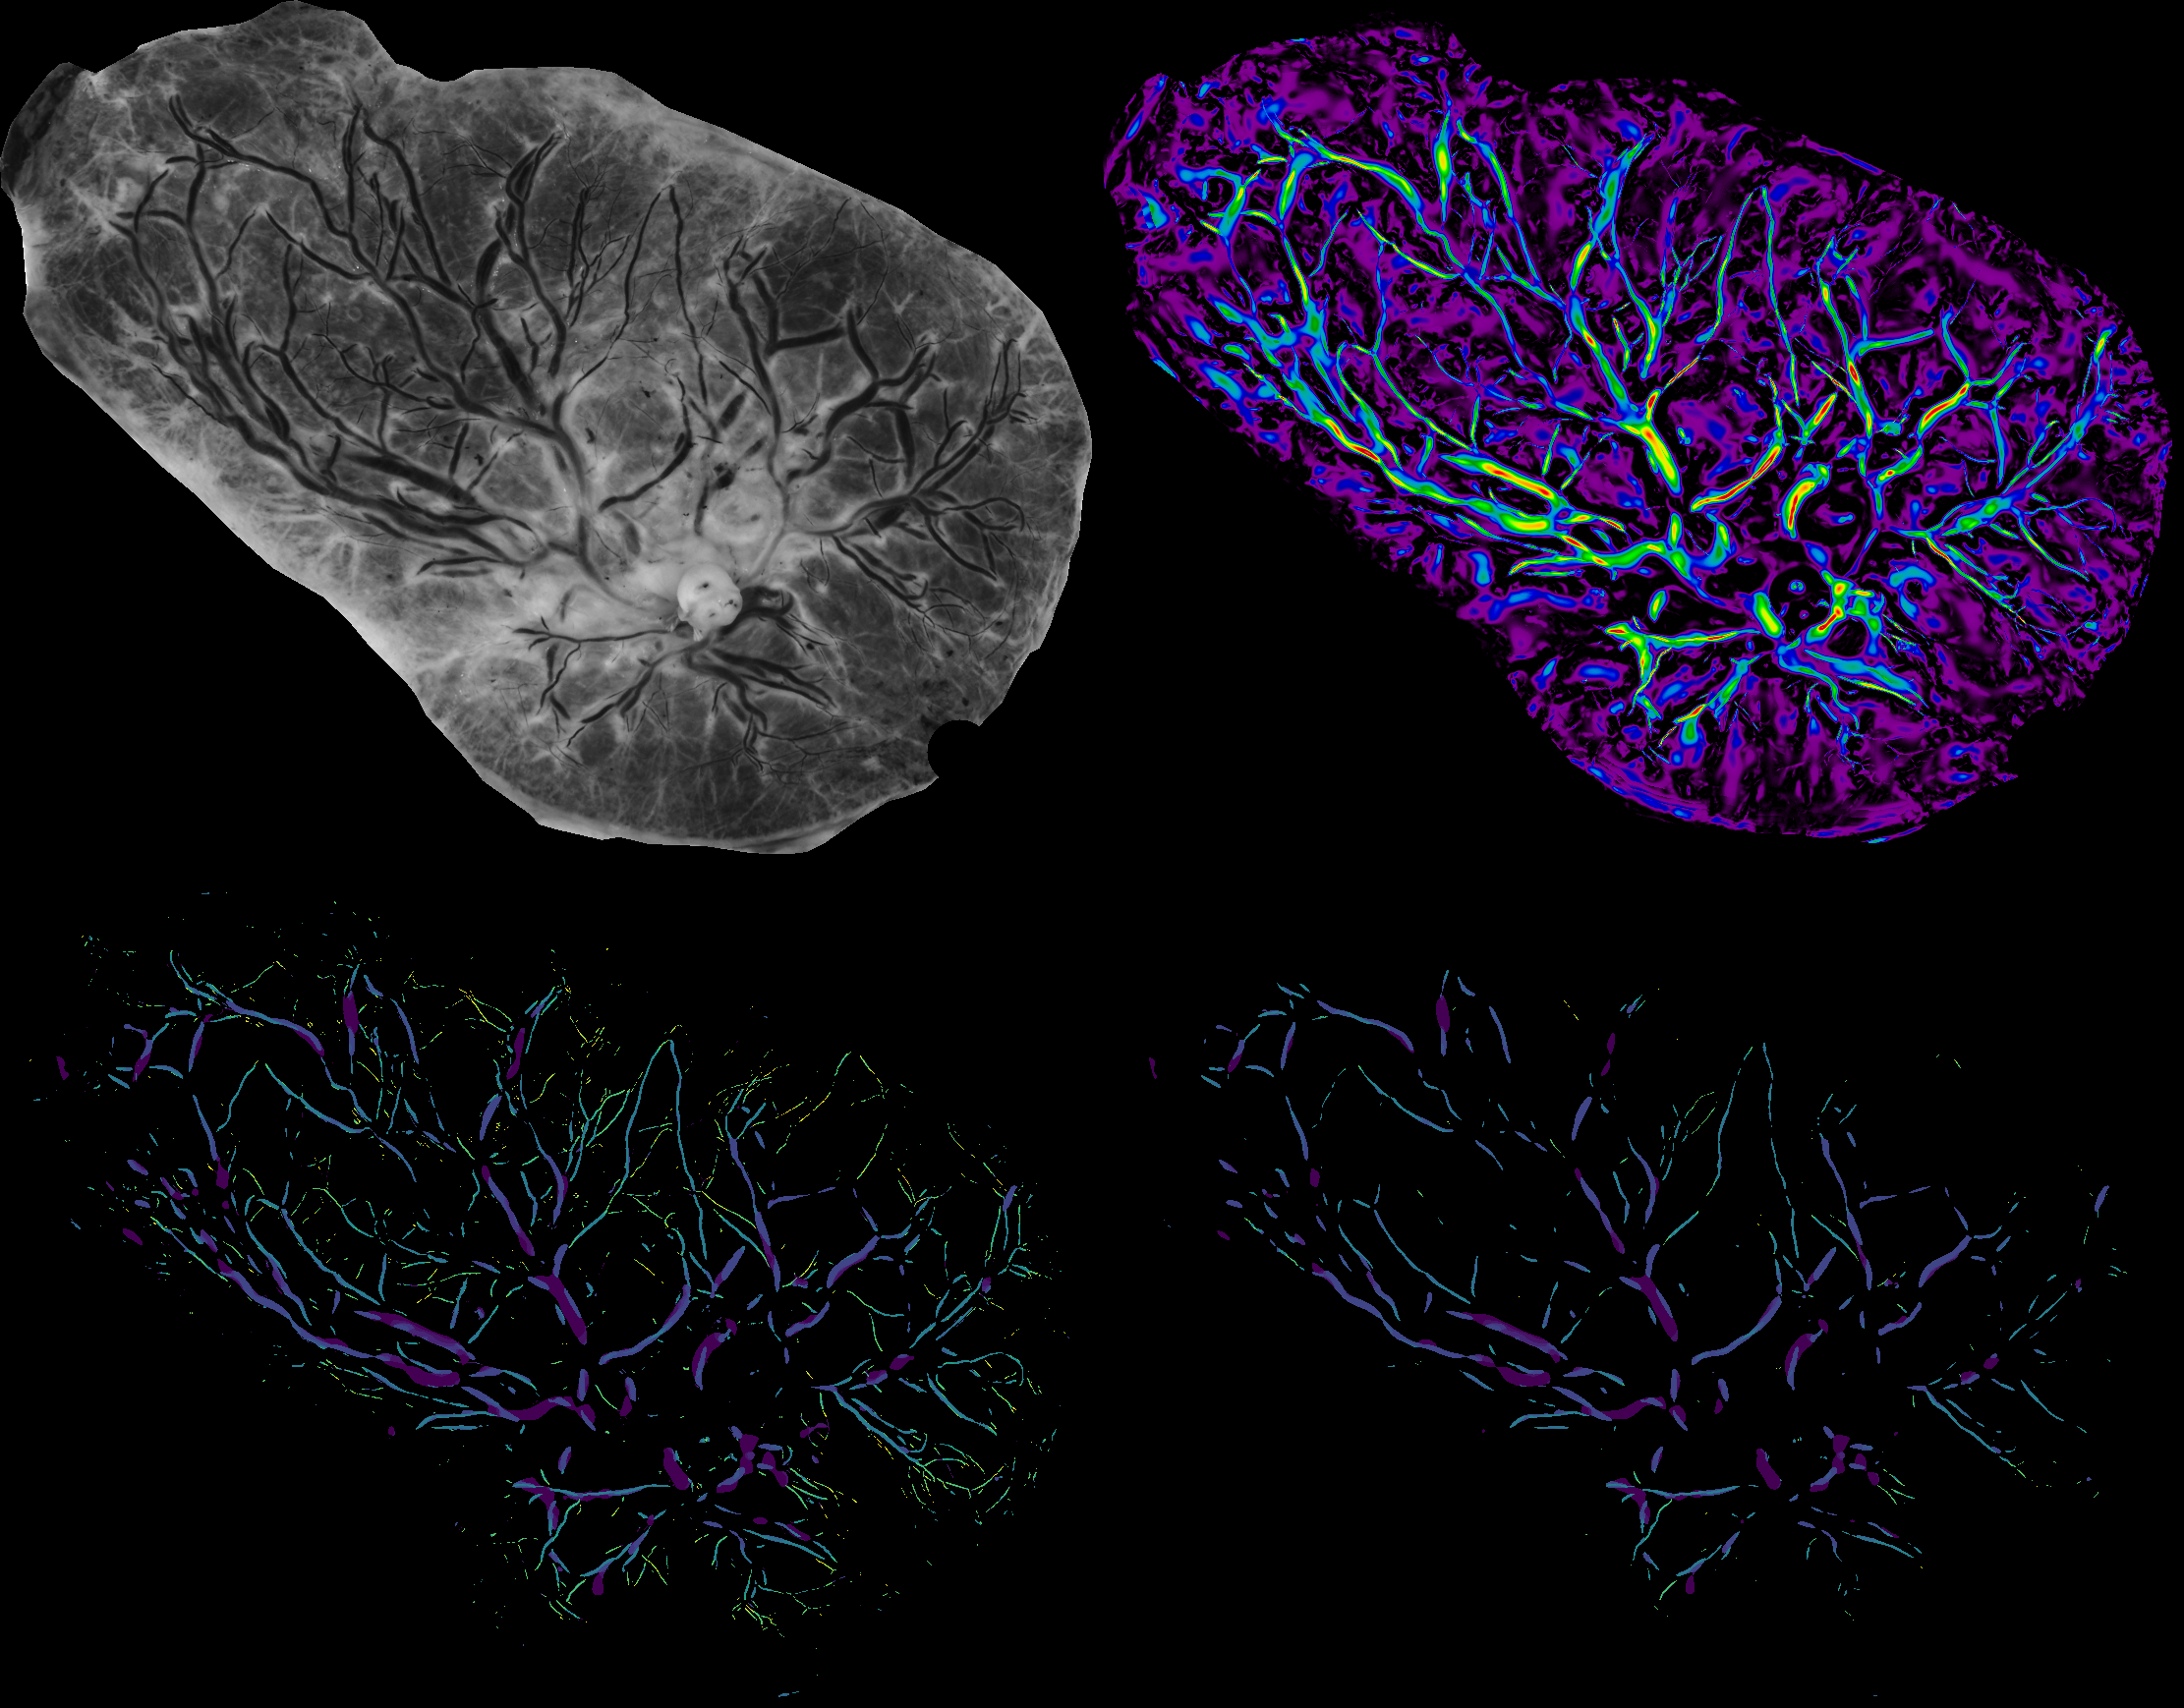
\includegraphics[width=\textwidth]{montage-T-BN0164923}
  \caption{Sample Multiscale Frangi output ($\beta=0.35$) with simple segmentation strategies (Example 1)}
  \label{fig:output-montage-example1}
\end{figure}

\begin{figure} \centering
  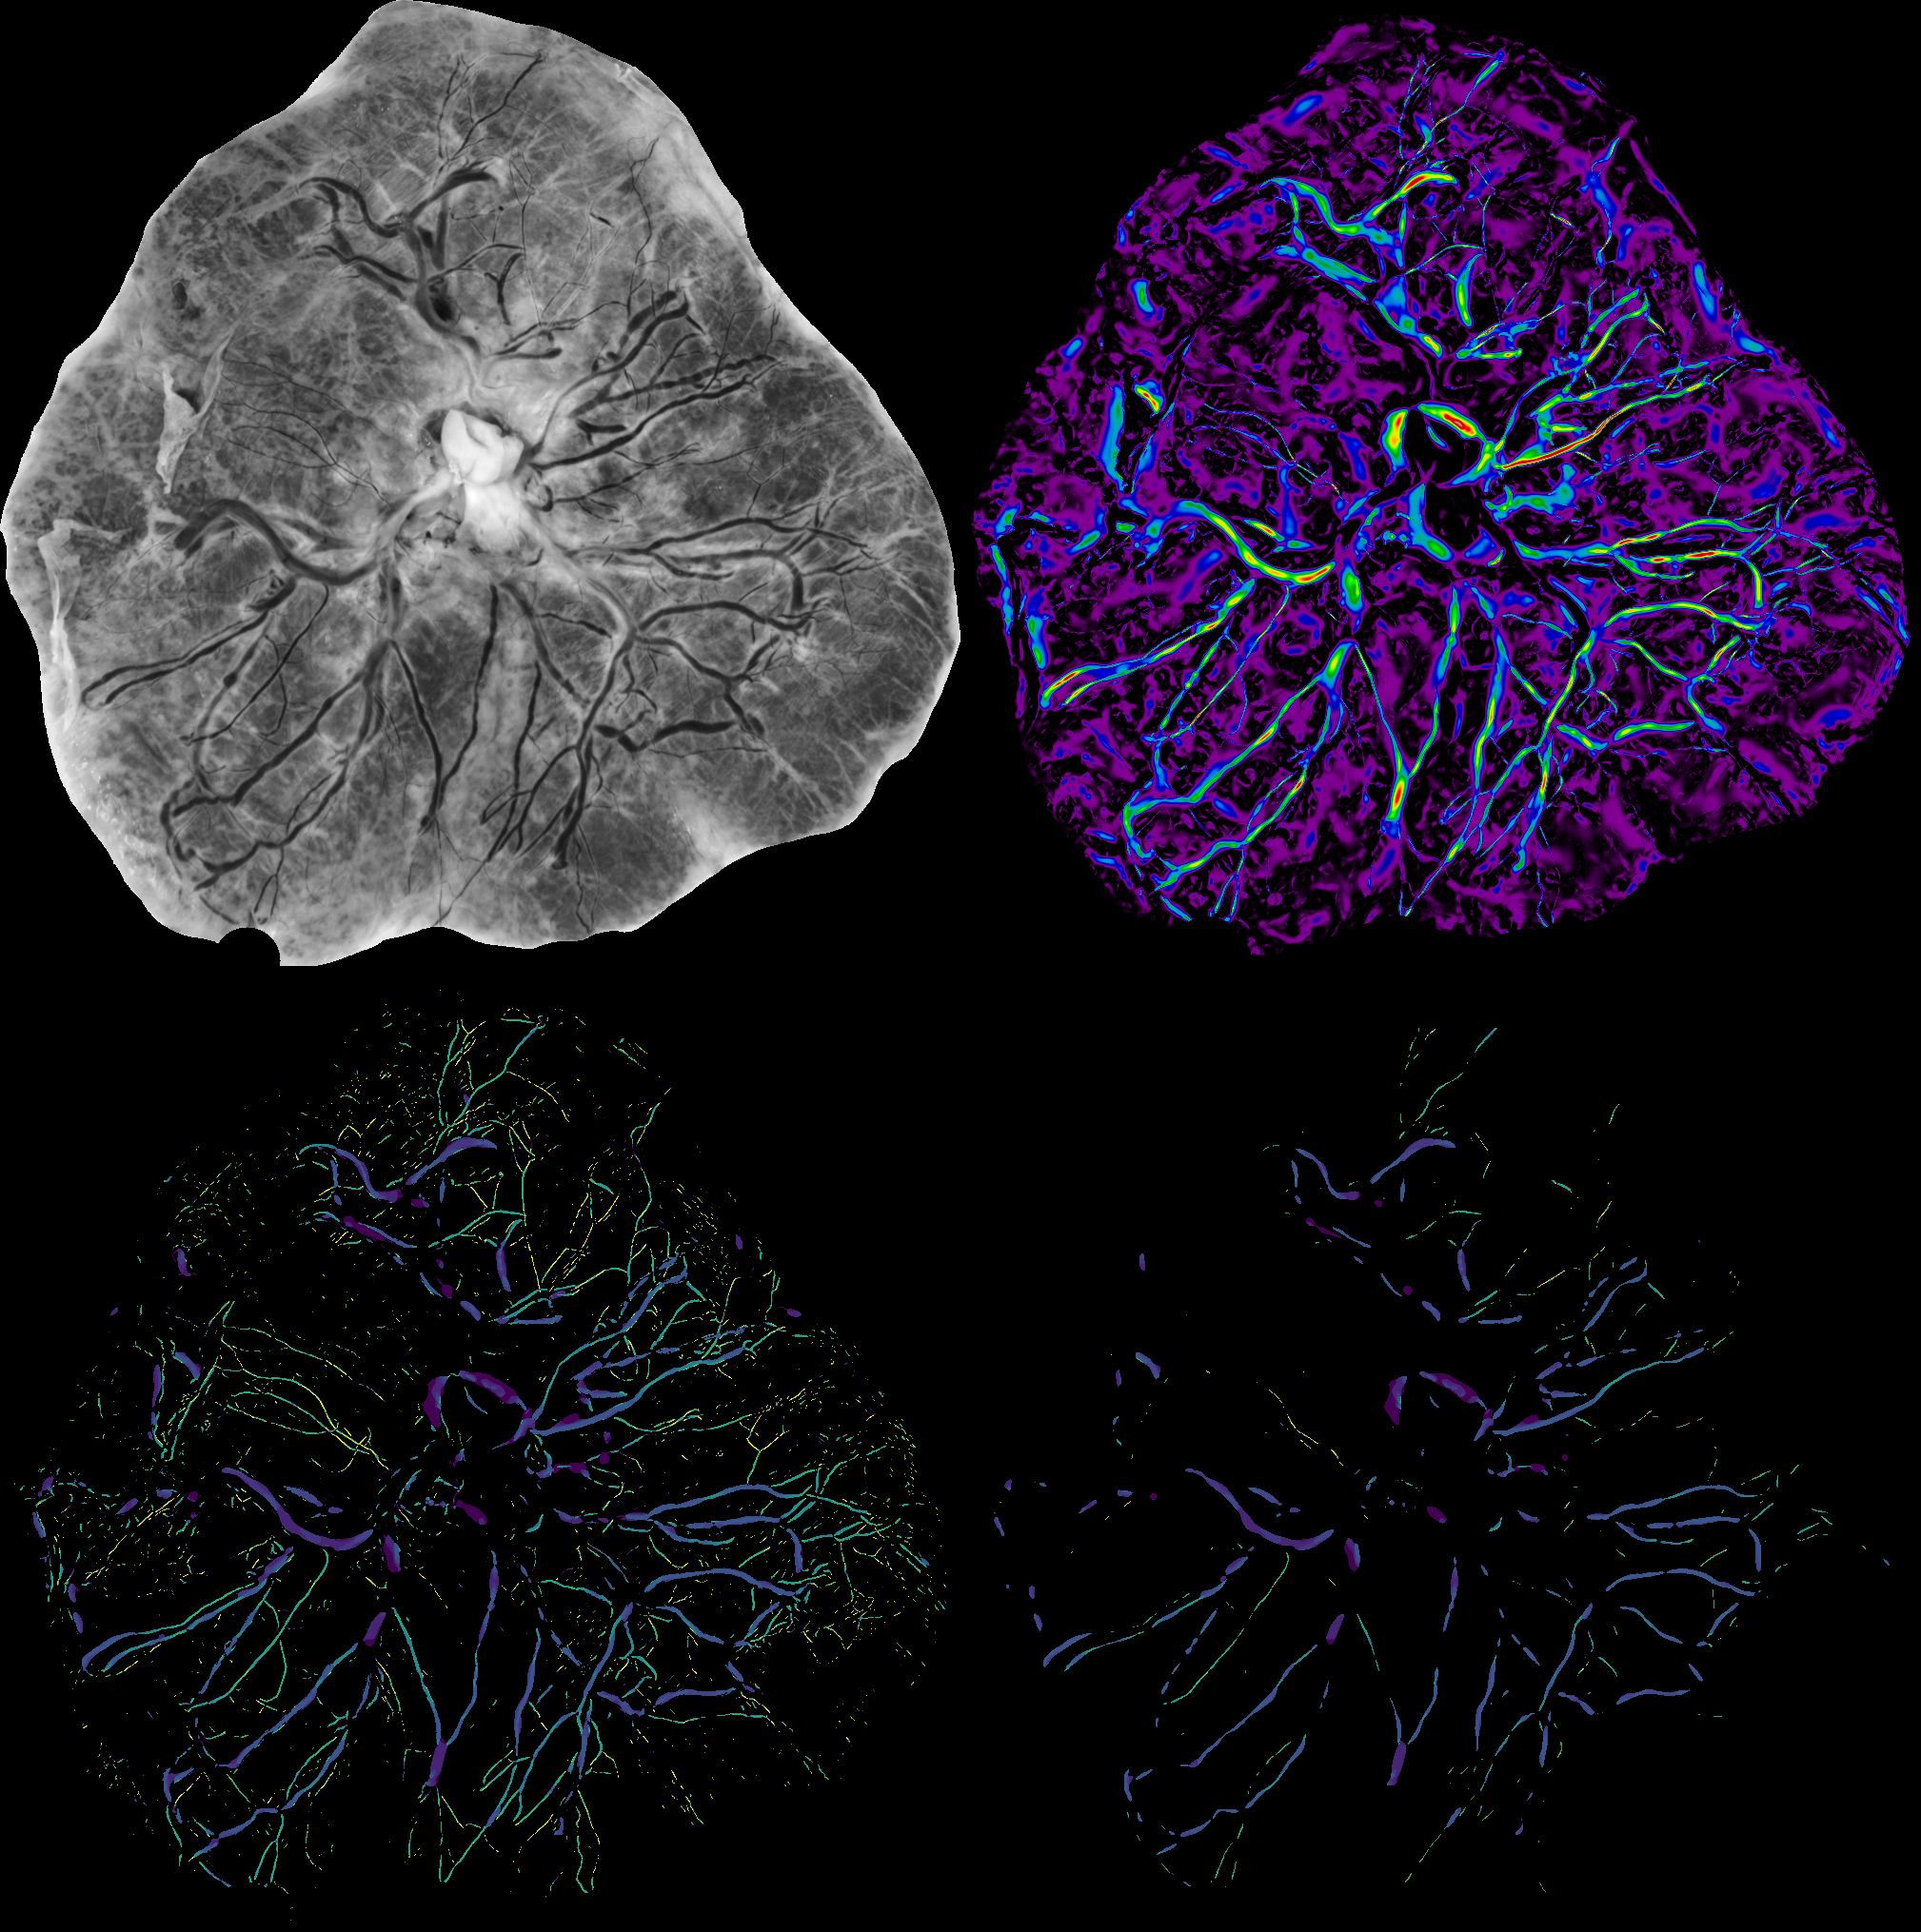
\includegraphics[width=\textwidth]{montage-T-BN0651415}
  \caption{Sample Multiscale Frangi output ($\beta=0.35$) with simple segmentation strategies (Example 2)}
  \label{fig:output-montage-example2}
\end{figure}


\subsection{Binary Classificaitons and the confusion matrix}

Here, we demonstrate the visual outputs produced by \texttt{extract\_NCS\_pcsvn.py}. This particular sample, BN4569506, is a relatively well-behaved sample, and segmentation was comparatively successful.

\begin{figure}
\centering
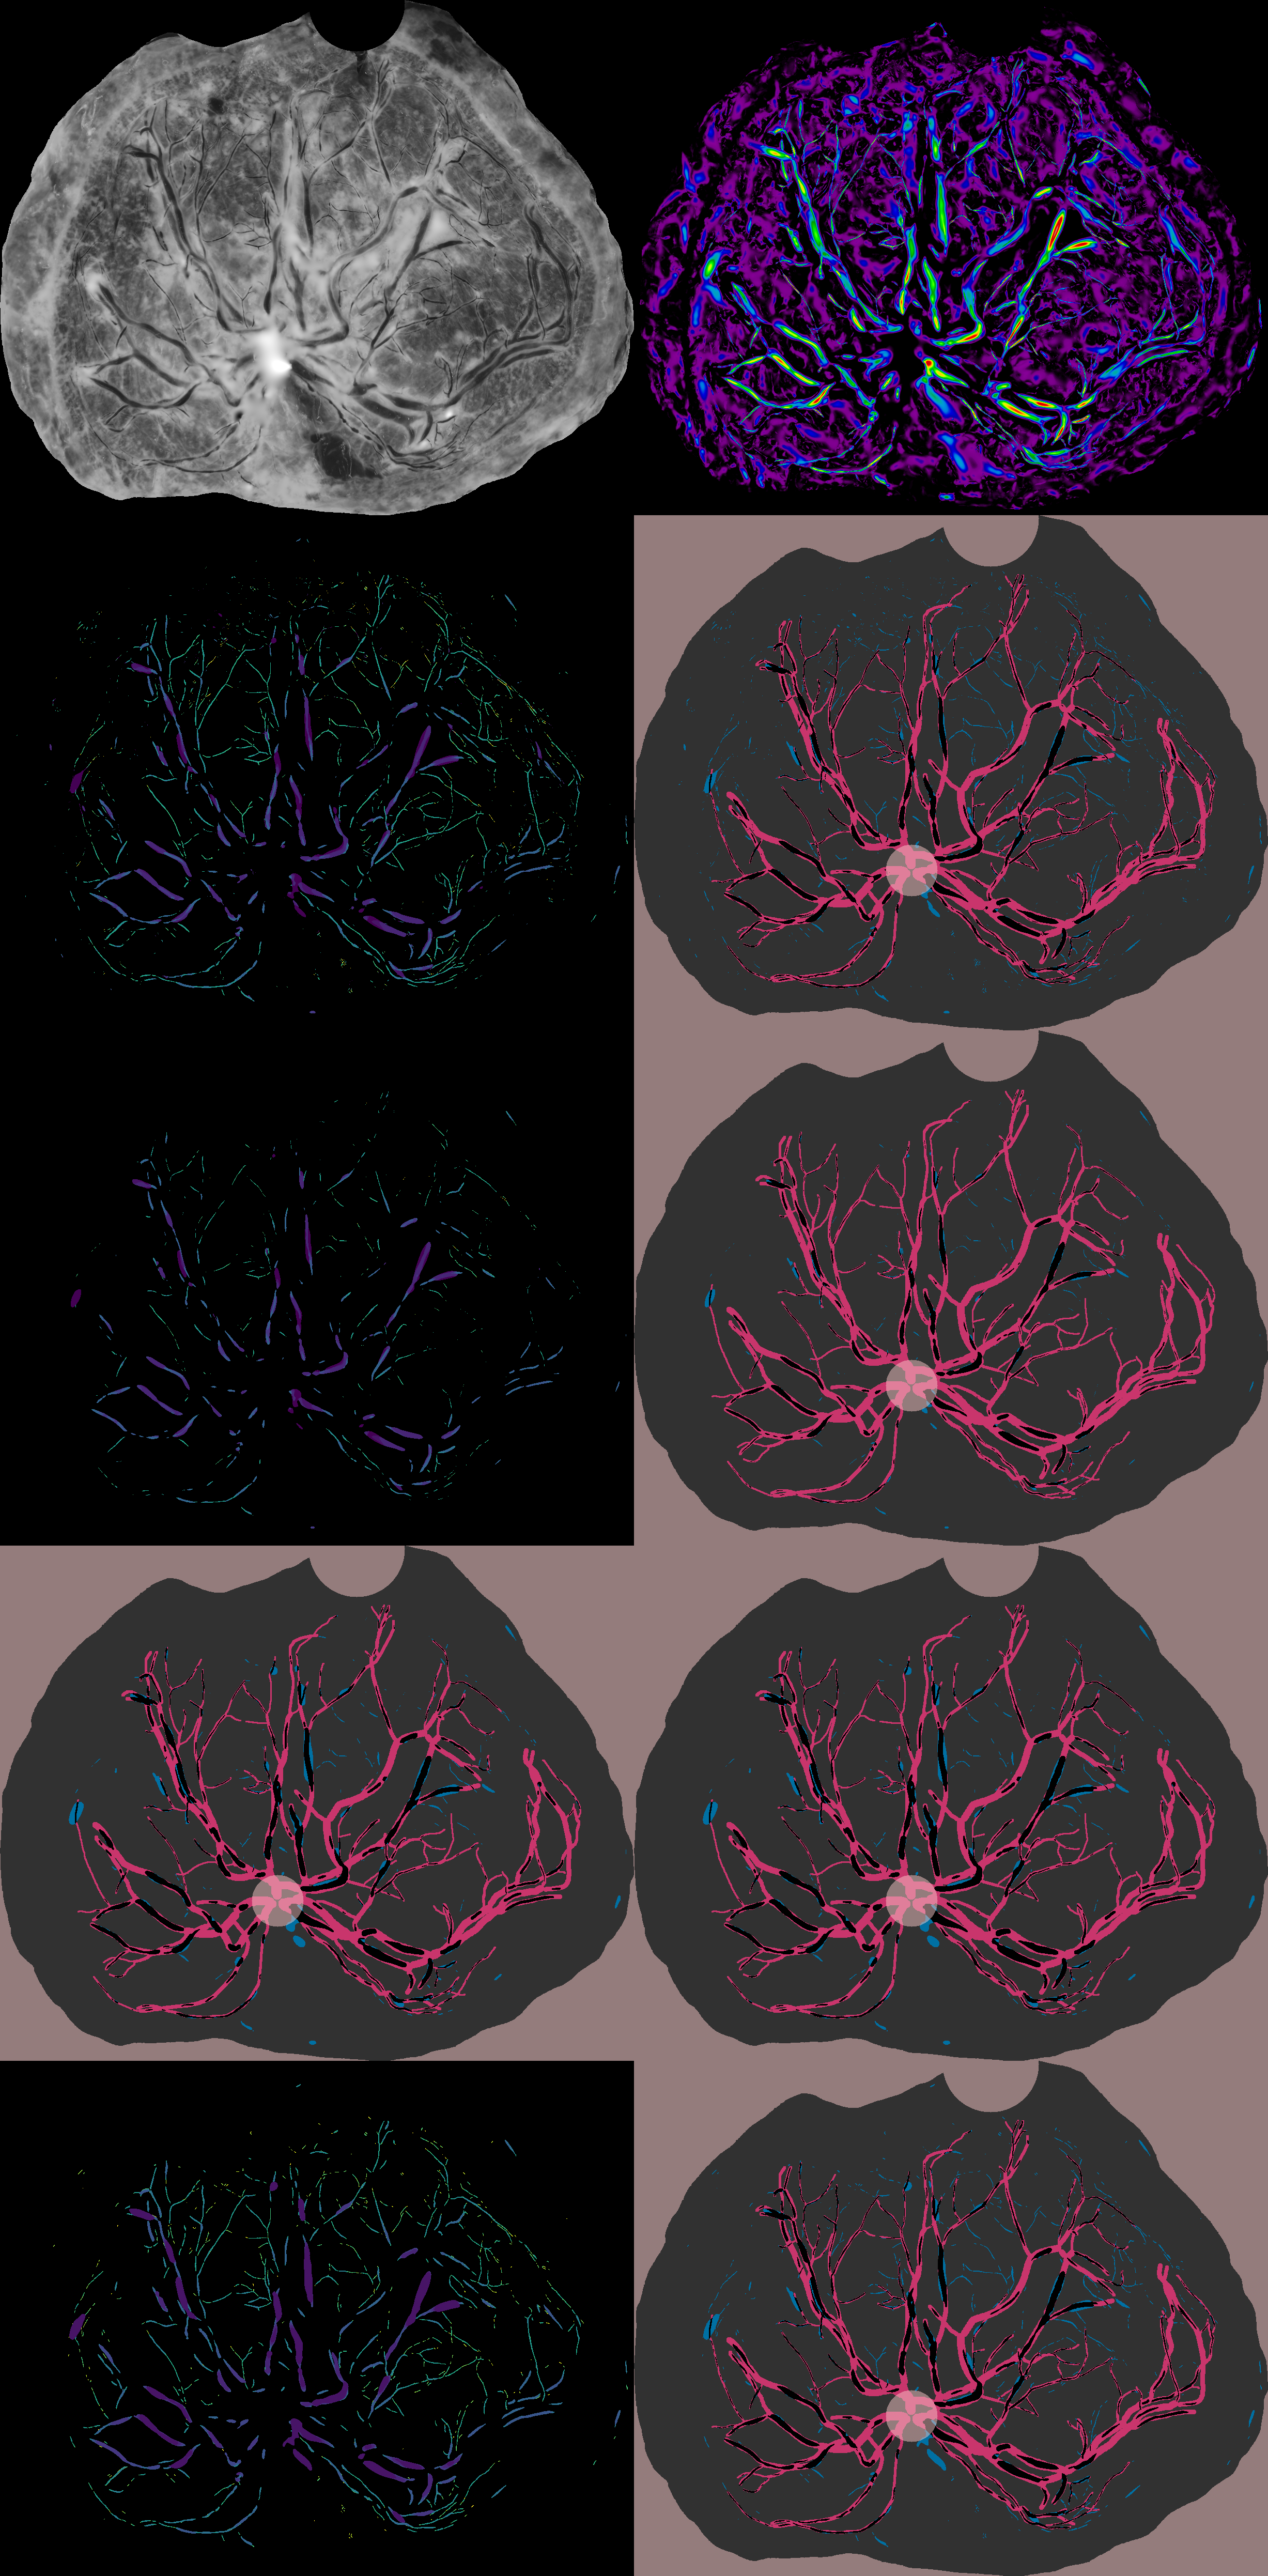
\includegraphics[height=\textheight]{BN4569506_output-montage}
\caption{Demonstration of postprocessing techniques}
  \end{figure}

There are 
use MCC \cite{mcc-original-paper}



\section{Variations in the Data Set and Imperfections of the Ground Truth} \label{sec:NCS-dataset-issues}

Sometimes the output doesn't agree with the trace, i.e. ``the ground truth'' is not 100\% correct.
sometimes either there's a false negative (reported) but something just wasn't traced in the original  1602443.

\begin{figure} \centering
  \subfloat{
  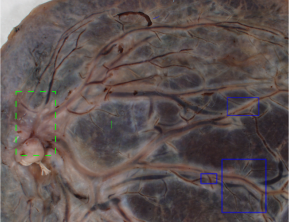
\includegraphics[width=0.5\textwidth]{T-BN0392644_inset}
}
\subfloat{
  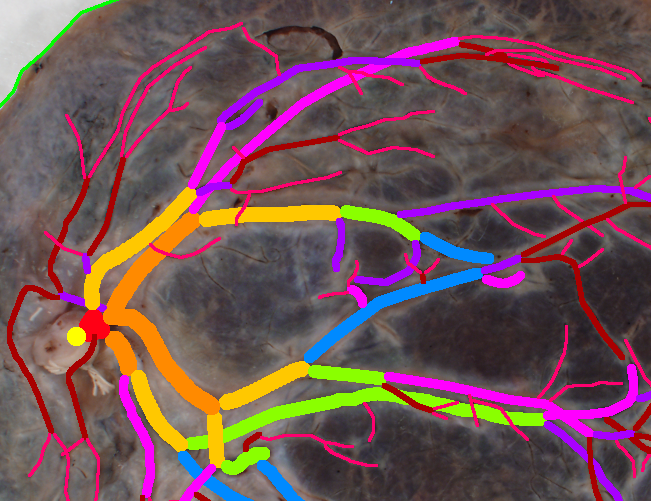
\includegraphics[width=0.5\textwidth]{T-BN0392644_inset_ctrace}
} \\
\subfloat{
  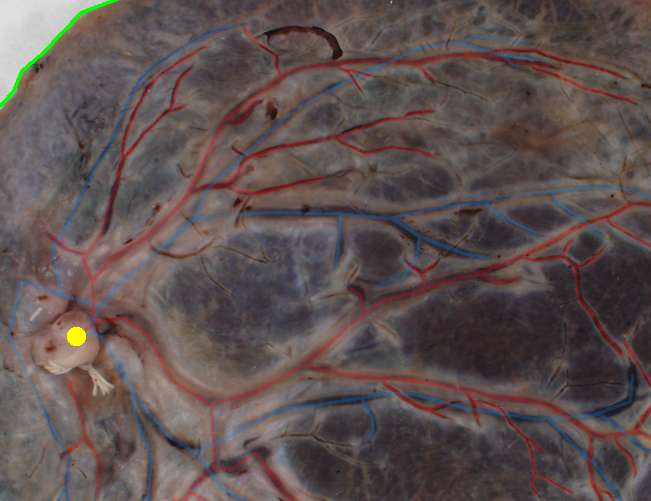
\includegraphics[width=0.5\textwidth]{T-BN0392644_inset_sketches}
}
\subfloat{
  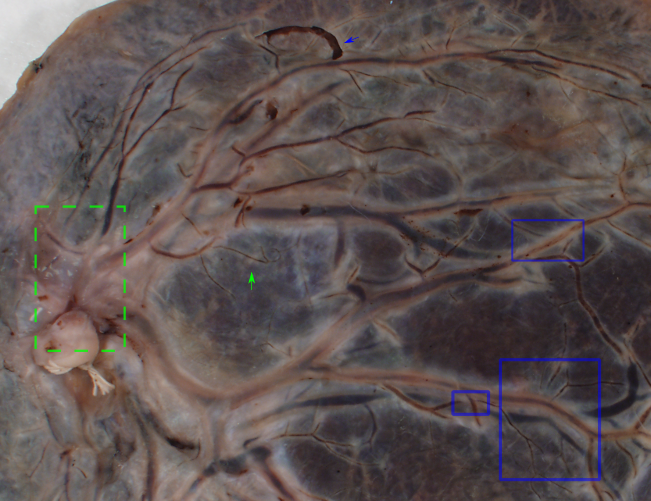
\includegraphics[width=0.5\textwidth]{T-BN0392644_inset_mark}
}
\caption{Issues with ground truth and sample quality}
\label{fig:groundtruth-samplequality}
\end{figure}

As seen in \cref{fig:groundtruth-samplequality}, there are several issues with the samples that will cause trouble in our efforts toward segmentation. Our represenative sample is BN0392644. The top left is the original (color) image, the top right is the full vessel width trace. The bottom left is a smaller skeletonization (sketch), where arteries are shown in red and veins are shown in blue. The bottom right figure contains some annotations. At the top, a blue arrow indicates a large curvilinear patch of dried blood that is not part of the vascular network. The green arrow in the middle indicates some vessels that are too small for the diameter binning and are thus not reported. We will see later that our Frangi result perfectly captures these, yet they will be reported as a false positive since they are not part of the tracing. However, there are other vessels of similar visual width in this same inset that are traced. In blue boxes (and in many other spots) the vessels cross each other. The border around these will prevent us from being able to extract the vessel directly. In the green dotted box, a major arterial and a major venous branch each connect to the umbilical cord insertion point. Whereas the arterial branch (on the right) can be seen, it will not be reported by the Frangi filter, since those points are not darker relative to the background. You can also see how much variation there is as you look along a blood vessel. There are some areas where the Frangi filter will have a very limited response. 



\begin{enumerate}
\item Collar is stupid and should really be considered like a error in marking the perimeter. Throw these away or edit. Maybe make a section called discarded samples that's stupid but yeah.
\item Vessels suck sometimes. In the portion above, 1602443, there's a random blood clot which gets identified at large $\sigma$. But also the small forked shaped thing which is obviously a vessel doesn't get defined.
\item Too much blood (not enough?? no idea) is left in the vessels. leading to the weird white border around some vessels. you could identify these along with black center and combine them somehow. no idea.Also, holy shit, some of the white vessel ``sleeves'' ARE identified in the tracing, and some aren't. Find an example of this and whine about it.
\item Umbillical cord insertion point is stupid and obscures a lot. The tracer guesses but there's no real guiding principle AFAIK..
\item Small vessels aren't accounted for at all. Not sure how to coincide measurement in terms of scale space anymore, but should figure out how to cut off those values before running MCC metric.
\end{enumerate}





\section{Results}
\begin{table}
\begin{tabular}{lrrrr}
  {} &  PF (q=95) &  FA (alpha=0.4) &  RW &  PS \\
  \hline
  MCC                  &                     0.505366 &                     0.434502 &      0.511190 &          0.505440 \\
  \% skeltrace coverage &                     0.498603 &                     0.306664 &      0.411479 &          0.527201 \\
  precision            &                     0.857878 &                     0.906386 &      0.821095 &          0.879843 \\
\end{tabular}
\caption{various metrics for gauging success of Frangi thresholding demos}
\end{table}


%\begin{itemize}
%	\item Relationship between traced pixelwidths vs the scale they were pulled from.
%	\item Frangi behavior at max scale length and if there's anything that gets too large (related to first derivatives maybe?
%	\item calculate the actual weingarten map eigenvectors (although this is
%	probably gonna be very fake in a discrete sense).
%	\item difference between using green channel and non-green channel.
%\end{itemize}

\begin{figure}[p]
    \centering
  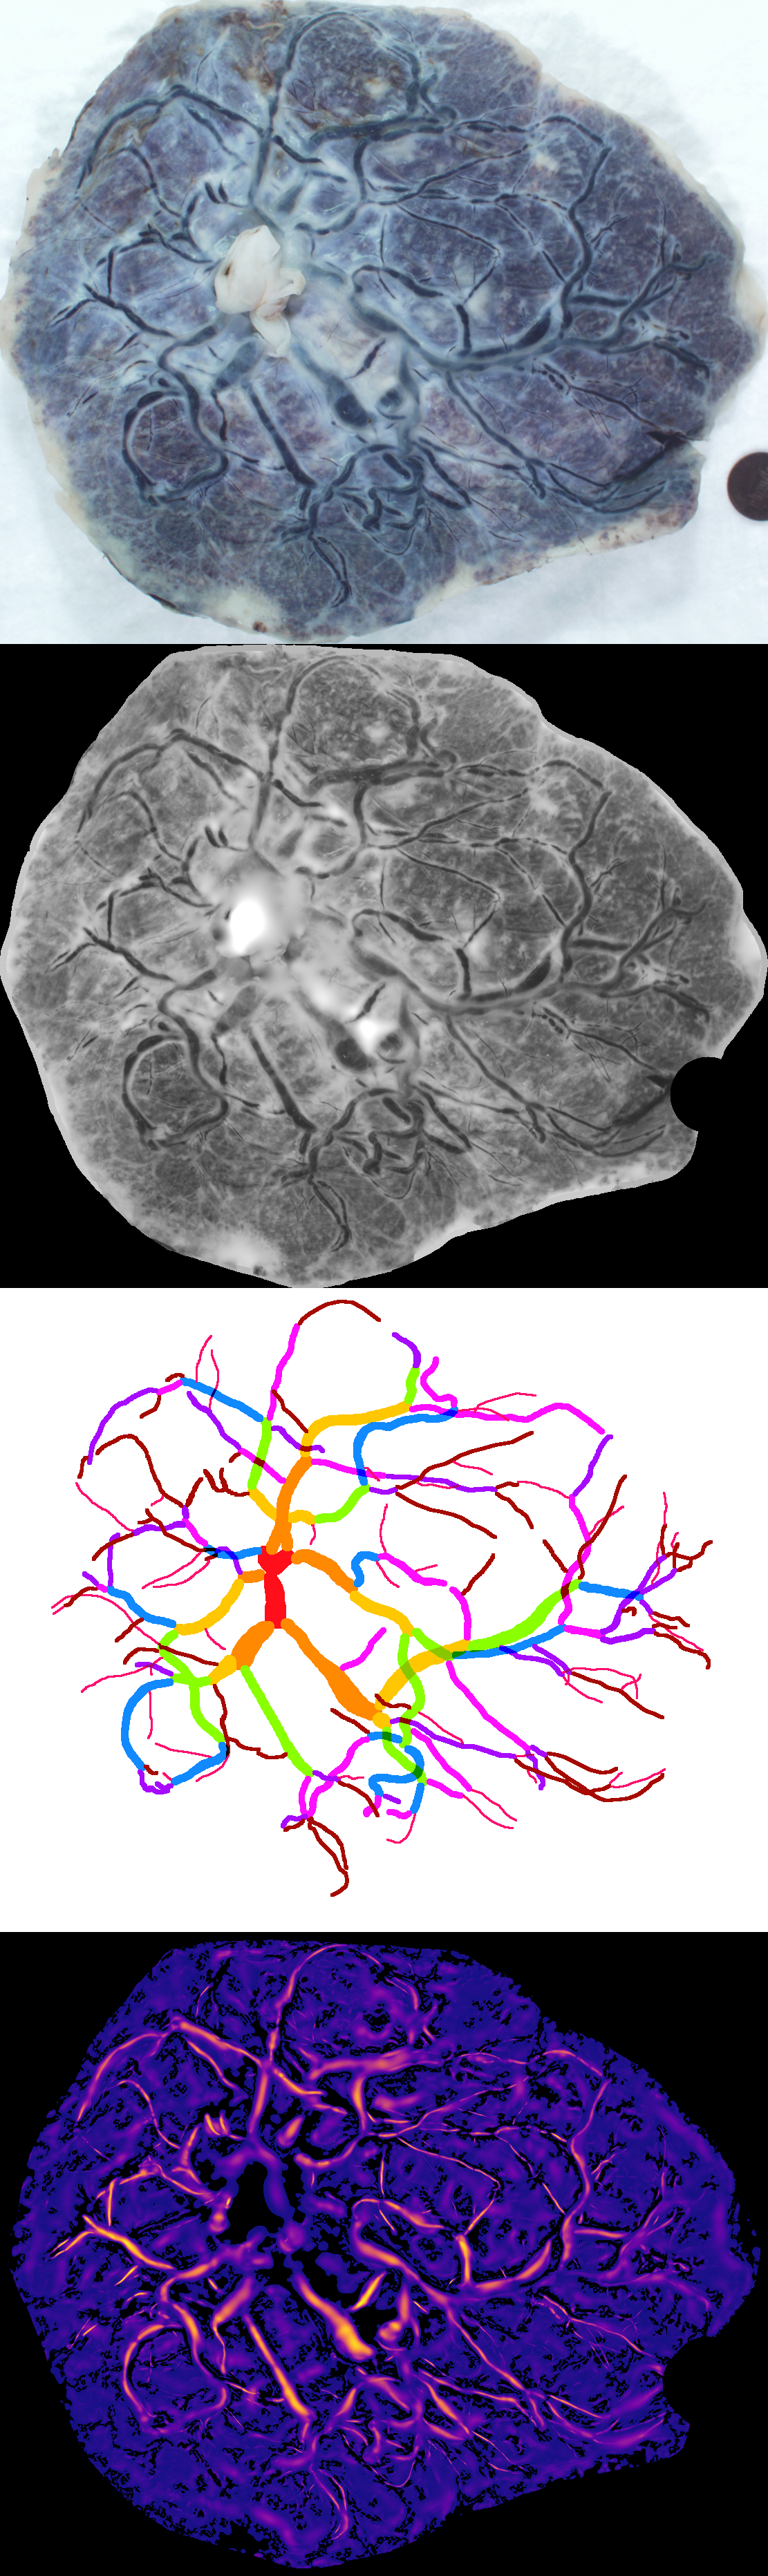
\includegraphics[height=\textheight]{M1-T-BN2050224}
\end{figure}
\quad
\begin{table}[p]
    \begin{small}
  \begin{tabular}{l|r|r|r}
    n  & $\sigma_n$  &  $\alpha_p$  &  $\max(V_\sigma)$ \\
    \hline
    0  &   0.3535 &  0.0547 &  0.986\\
    1  &   0.4243 &  0.0590 &  0.979\\
    2  &   0.5092 &  0.0654 &  0.970\\
    3  &   0.6110 &  0.0765 &  0.973\\
    4  &   0.7333 &  0.0892 &  0.988\\
    5  &   0.8801 &  0.0962 &  0.991\\
    6  &   1.0562 &  0.1082 &  0.991\\
    7  &   1.2676 &  0.1308 &  0.970\\
    8  &   1.5212 &  0.1669 &  0.973\\
    9  &   1.8256 &  0.2232 &  0.978\\
    10 &   2.1909 &  0.2925 &  0.984\\
    11 &   2.6294 &  0.3196 &  0.968\\
    12 &   3.1555 &  0.3269 &  0.994\\
    13 &   3.7869 &  0.3558 &  0.998\\
    14 &   4.5447 &  0.4058 &  0.999\\
    15 &   5.4542 &  0.3764 &  0.963\\
    16 &   6.5456 &  0.3184 &  0.950\\
    17 &   7.8553 &  0.3047 &  0.958\\
    18 &   9.4272 &  0.3287 &  0.916\\
    19 &  11.3137 &  0.3524 &  0.916\\
    \end{tabular}
\end{small}
  \caption{Vesselness scores and percentile thresholds}
\end{table}
\clearpage


\begin{figure}[p] \centering
 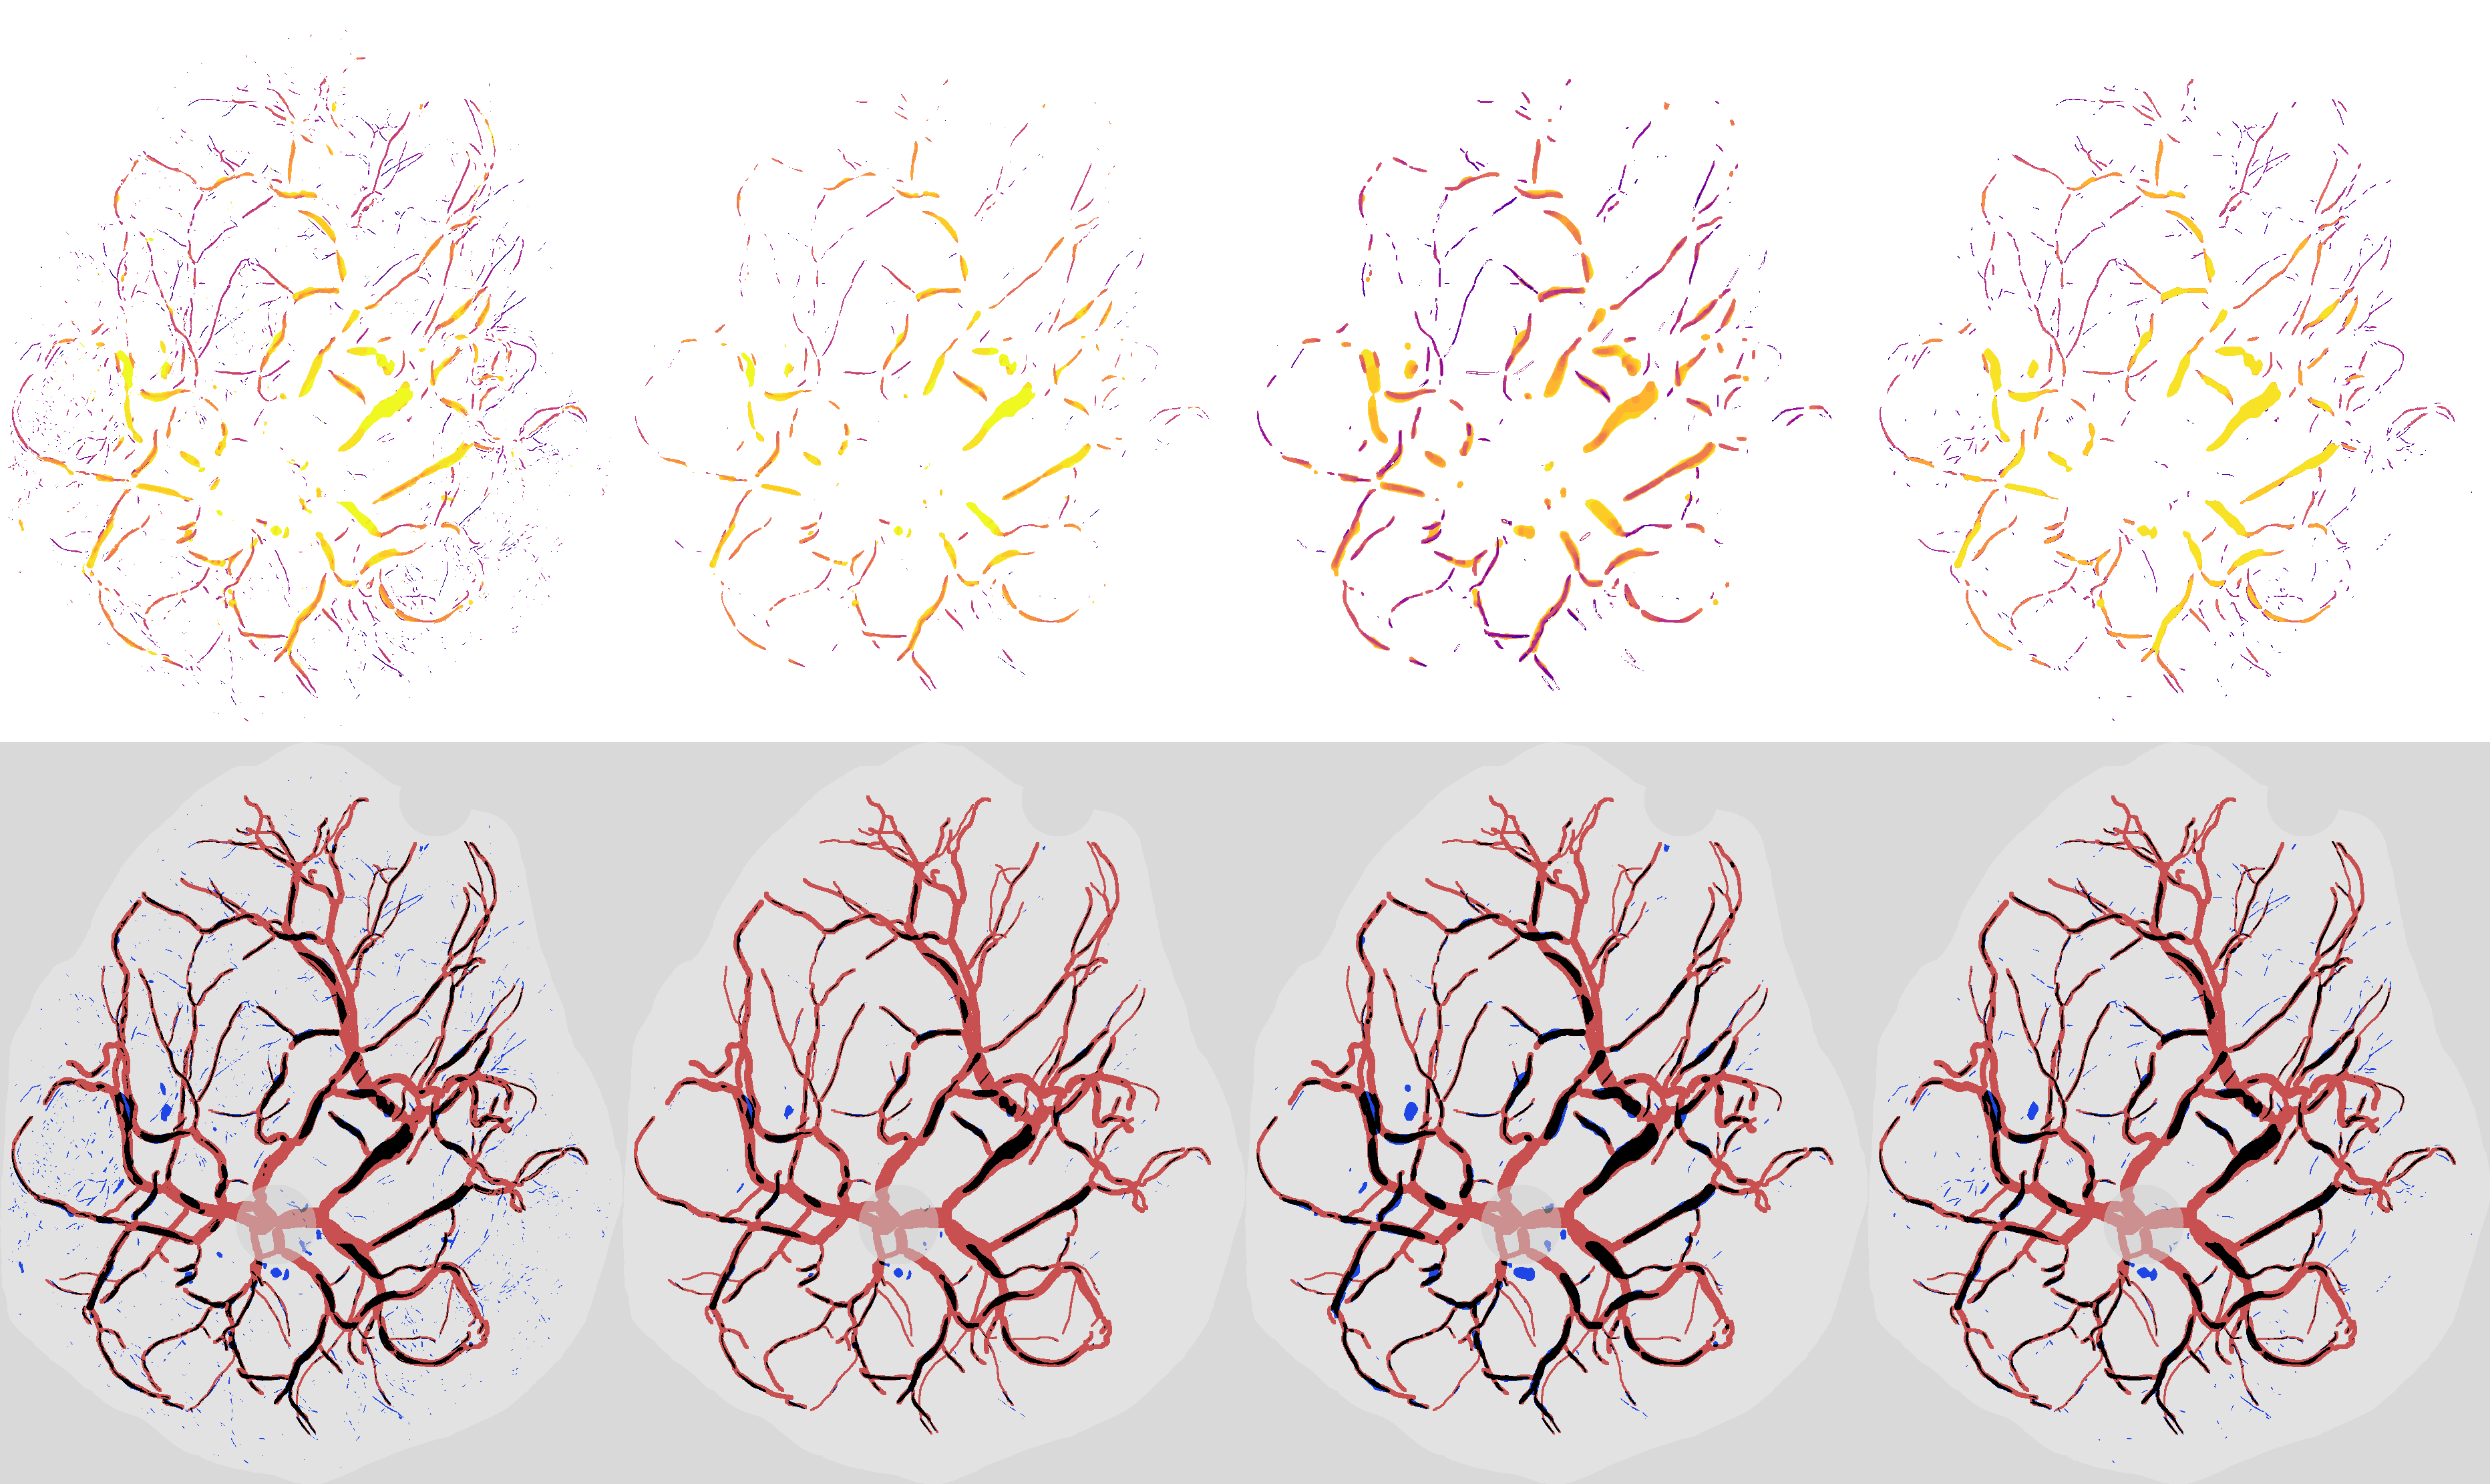
\includegraphics[width=\linewidth]{M2-T-BN2050224}
 \caption{Sample of Frangi-based Segmentation Methods (pt. 2)}
  \end{figure}

\begin{table}[p]\centering
  \begin{tabular}{l|rrrr}
    {} &        PF &        FA &        RW &        PS \\
    \hline
    MCC           &  0.4872 &  0.4208 &  0.5249 &  0.4877 \\
    %\hline
    skel coverage &  0.5085 &  0.3245 &  0.4493 &  0.4650 \\
    %\hline
    precision     &  0.8044 &  0.9472 &  0.8858 &  0.8697 \\
  \end{tabular}
\caption{Scores for merging techniques}
\end{table}

\begin{figure}[p]
  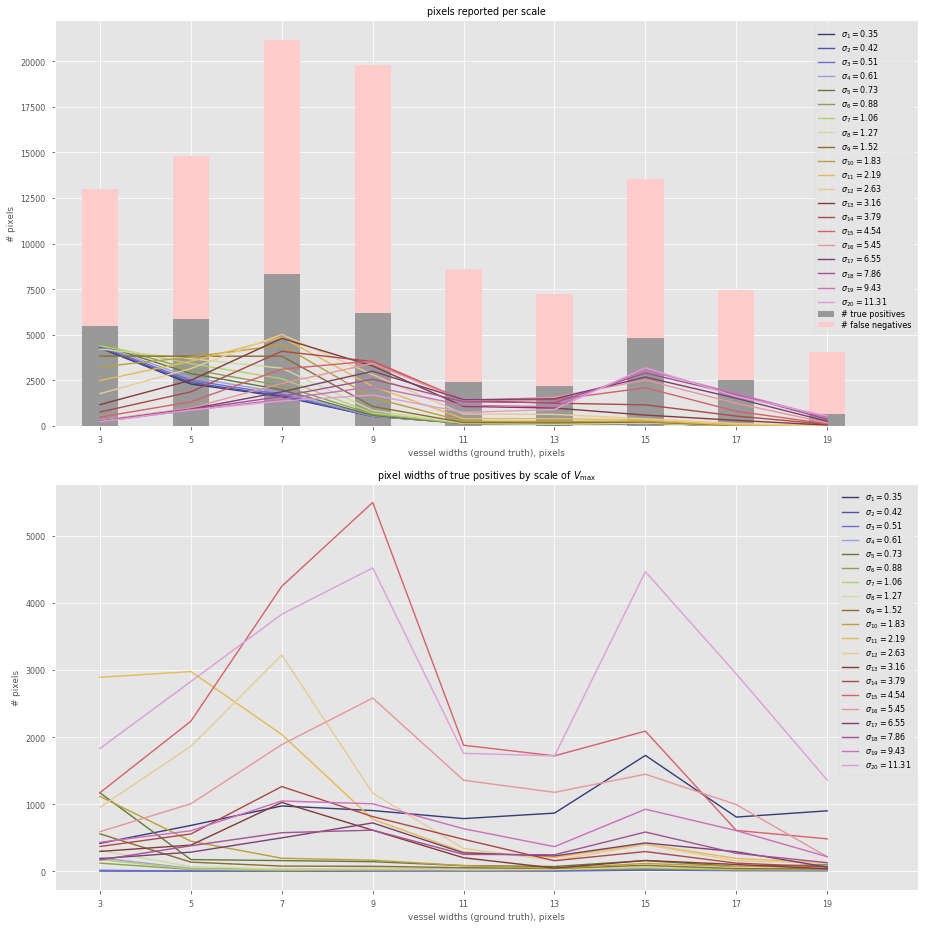
\includegraphics[width=\textwidth]{test-scale-width}
  \caption{Pixel Width of Ground Truth vs. Scale Length for True Positives}
\end{figure}

\begin{figure}[p]\centering
  \subfloat{
  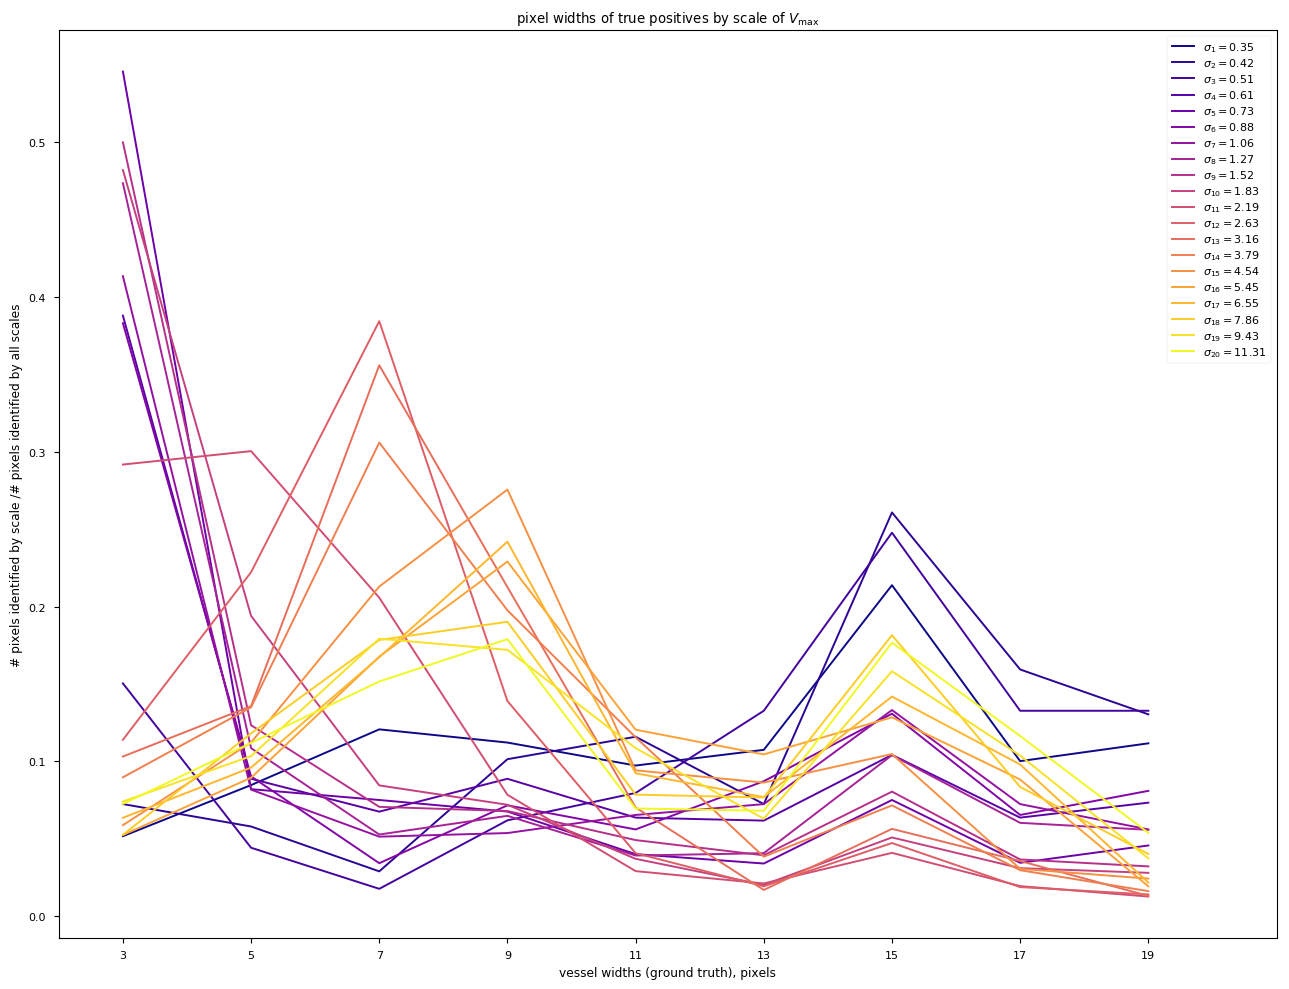
\includegraphics[width=0.85\textwidth]{Vmax_to_scale_normalized}
  }\\[-0.5cm]
  \subfloat{
  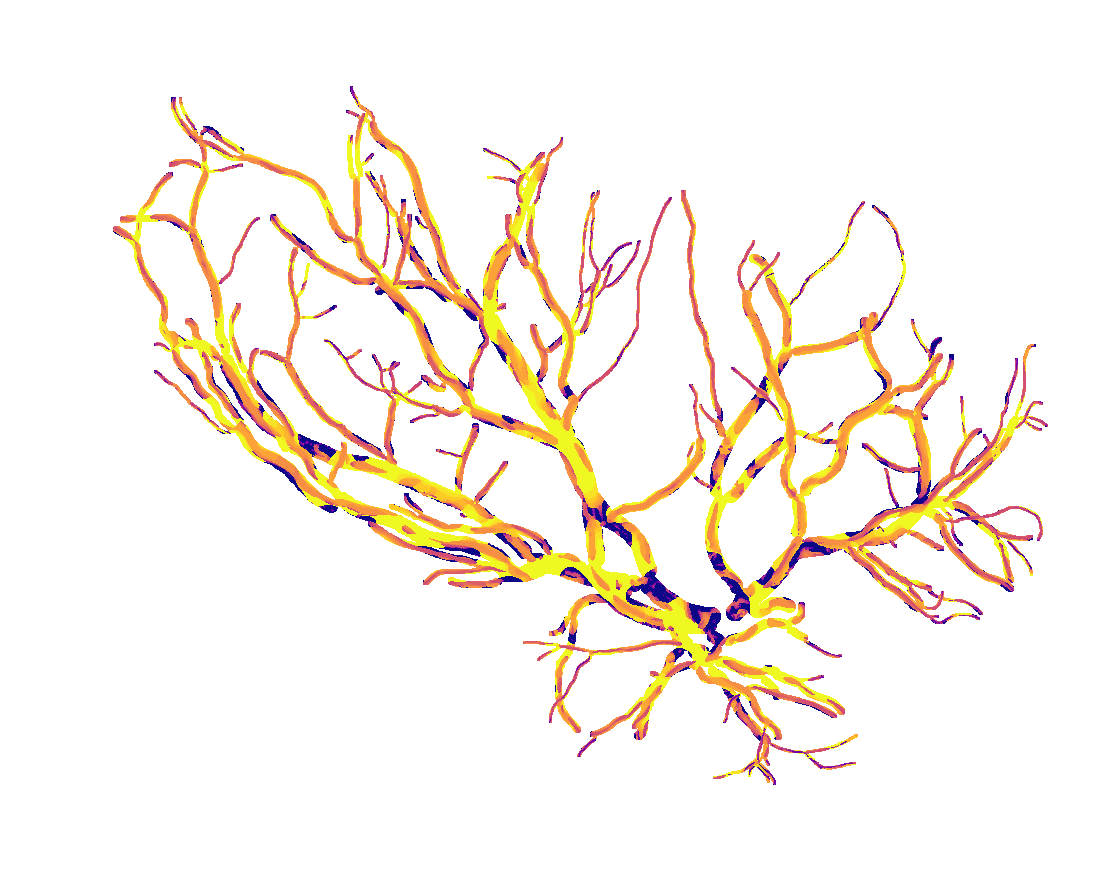
\includegraphics[width=0.85\textwidth]{frangi_argmax-trace}
  }
  \caption{Scale of maximum Frangi score for true positives and false negatives}
\end{figure}

\begin{figure}[p]\centering
  \subfloat{
    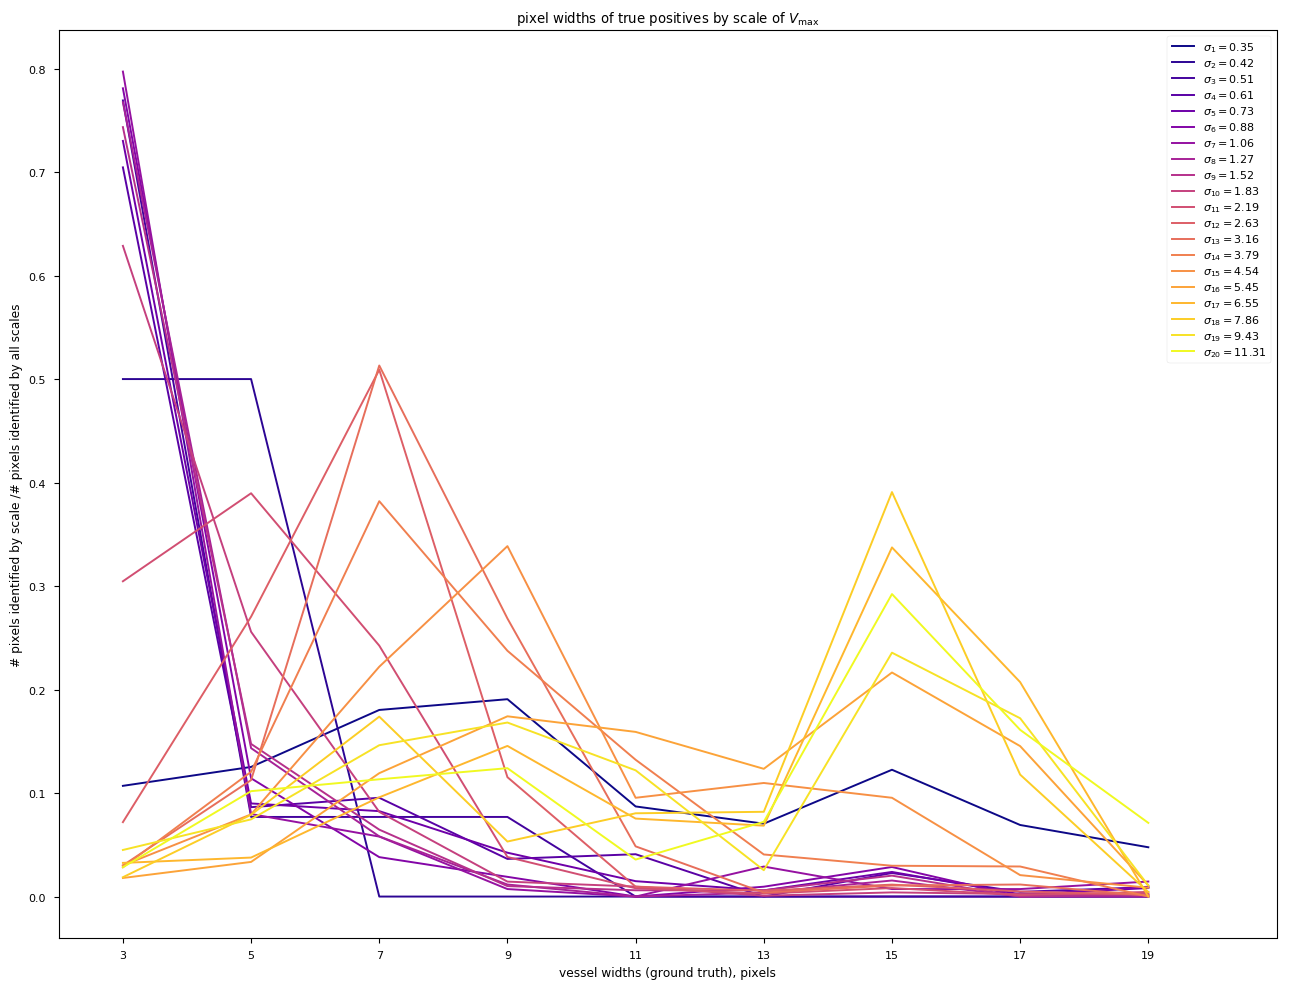
\includegraphics[width=0.85\textwidth]{Vmax_to_scale_normalized_with_approx}
  }\\[-0.5cm]
  \subfloat{
    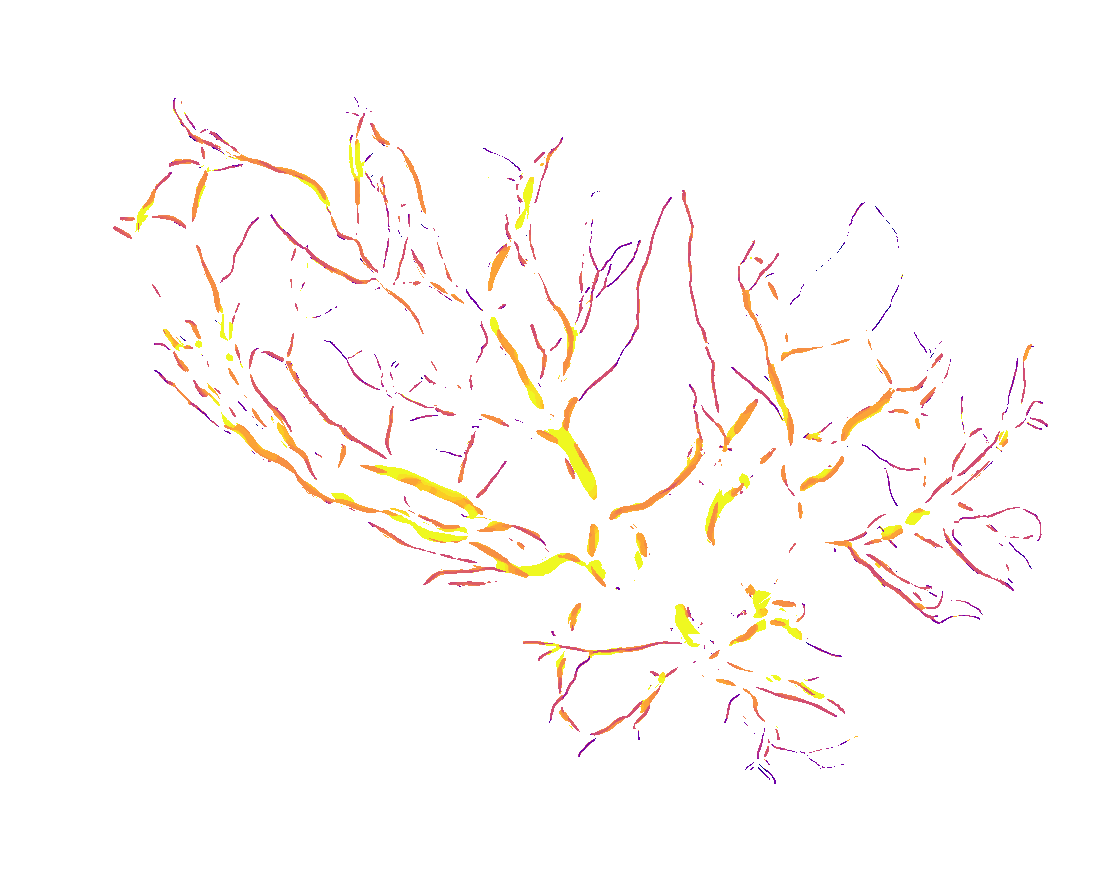
\includegraphics[width=0.85\textwidth]{frangi_argmax-trace-approx}
  }
  \caption{Scale of maximum Frangi score for true positives only (percentile filtering)}
\end{figure}
